
%(BEGIN_QUESTION)
% Copyright 2011, Tony R. Kuphaldt, released under the Creative Commons Attribution License (v 1.0)
% This means you may do almost anything with this work of mine, so long as you give me proper credit

I dette SCADA-systemet kommuniserer en ``master''-PLC (MTU) med flere ``slave''-PLC-er (RTU-er) via radio med Modbus-protokoll.  Hver PLC kommuniserer med sin radiotransceiver via en kort RS-232-seriellkabel.  Illustrasjonen er omtrent tegnet i skala med hensyn til avstandene mellom enhetene:

$$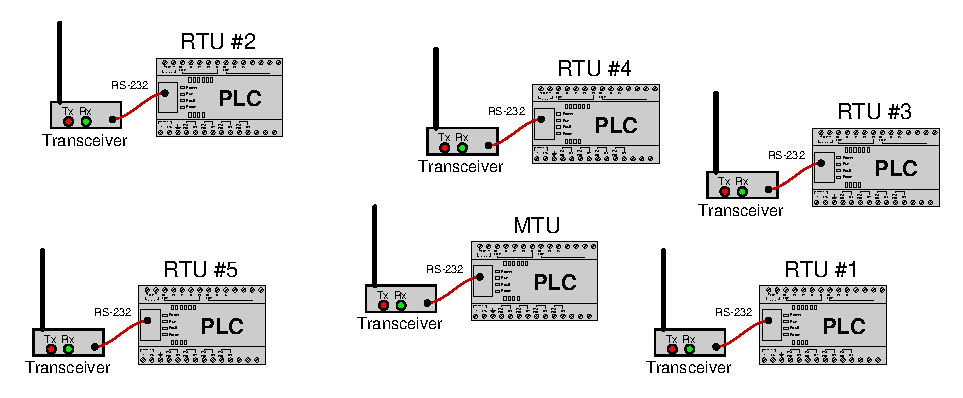
\includegraphics[width=15.5cm]{i00220x01.eps}$$

Dessverre er det et problem i dette systemet.  Ingen av RTU-ene kommuniserer med MTU-en.  Ved inspeksjon ser du at ``Tx''-indikatoren blinker på MTU-ens transceiverenhet, men ikke ``Rx''-indikatoren.

Identifiser sannsynligheten for hver spesifisert feil i dette systemet.  Vurder hver feil én om gangen (dvs. ingen samtidige feil), og avgjør om hver feil uavhengig kan forklare {\it alle} målinger og symptomer i dette SCADA-nettverket.

% No blank lines allowed between lines of an \halign structure!
% I use comments (%) instead, so that TeX doesn't choke.

$$\vbox{\offinterlineskip
\halign{\strut
\vrule \quad\hfil # \ \hfil & 
\vrule \quad\hfil # \ \hfil & 
\vrule \quad\hfil # \ \hfil \vrule \cr
\noalign{\hrule}
%
% First row
{\bf Feil} & {\bf Mulig} & {\bf Umulig} \cr
%
\noalign{\hrule}
%
% Another row
Skadet antenne på MTU &  &  \cr
%
\noalign{\hrule}
%
% Another row
Skadet antenne på RTU \#4 &  &  \cr
%
\noalign{\hrule}
%
% Another row
PLC stoppet (ikke kjørende) på MTU &  &  \cr
%
\noalign{\hrule}
%
% Another row
Radiotransceiver avslått på RTU \#4 &  &  \cr
%
\noalign{\hrule}
%
% Another row
``TD''-leder brutt i RS-232-kabelen på MTU &  &  \cr
%
\noalign{\hrule}
%
% Another row
``RD''-leder brutt i RS-232-kabelen på MTU &  &  \cr
%
\noalign{\hrule}
%
% Another row
PLC-baudrate satt feil på RTU \#4 &  &  \cr
%
\noalign{\hrule}
%
% Another row
PLC-baudrate satt feil på MTU &  &  \cr
%
\noalign{\hrule}
%
% Another row
Modbus-modus (RTU/ASCII) satt feil på RTU \#4 &  &  \cr
%
\noalign{\hrule}
%
% Another row
Modbus-modus (RTU/ASCII) satt feil på MTU &  &  \cr
%
\noalign{\hrule}
%
% Another row
Fresnel-sone-interferens mellom MTU og RTU \#4 &  &  \cr
%
\noalign{\hrule}
} % End of \halign 
}$$ % End of \vbox

Til slutt: identifiser den {\it neste} diagnostiske testen eller målingen du ville gjort på dette systemet.  Forklar hvordan resultatet(-ene) av denne testen eller målingen hjelper deg med å finne plassering og/eller type feil videre.

\underbar{file i00220}
%(END_QUESTION)





%(BEGIN_ANSWER)

\noindent
{\bf Delvis svar:}

% No blank lines allowed between lines of an \halign structure!
% I use comments (%) instead, so that TeX doesn't choke.

$$\vbox{\offinterlineskip
\halign{\strut
\vrule \quad\hfil # \ \hfil & 
\vrule \quad\hfil # \ \hfil & 
\vrule \quad\hfil # \ \hfil \vrule \cr
\noalign{\hrule}
%
% First row
{\bf Feil} & {\bf Mulig} & {\bf Umulig} \cr
%
\noalign{\hrule}
%
% Another row
Skadet antenne på MTU &  &  \cr
%
\noalign{\hrule}
%
% Another row
Skadet antenne på RTU \#4 &  &  \cr
%
\noalign{\hrule}
%
% Another row
PLC stoppet (ikke kjørende) på MTU &  &  \cr
%
\noalign{\hrule}
%
% Another row
Radiotransceiver avslått på RTU \#4 &  & $\surd$ \cr
%
\noalign{\hrule}
%
% Another row
``TD''-leder brutt i RS-232-kabelen på MTU &  &  \cr
%
\noalign{\hrule}
%
% Another row
``RD''-leder brutt i RS-232-kabelen på MTU &  &  \cr
%
\noalign{\hrule}
%
% Another row
PLC-baudrate satt feil på RTU \#4 &  & $\surd$ \cr
%
\noalign{\hrule}
%
% Another row
PLC-baudrate satt feil på MTU &  &  \cr
%
\noalign{\hrule}
%
% Another row
Modbus-modus (RTU/ASCII) satt feil på RTU \#4 &  & $\surd$ \cr
%
\noalign{\hrule}
%
% Another row
Modbus-modus (RTU/ASCII) satt feil på MTU & $\surd$ &  \cr
%
\noalign{\hrule}
%
% Another row
Fresnel-sone-interferens mellom MTU og RTU \#4 &  &  \cr
%
\noalign{\hrule}
} % End of \halign 
}$$ % End of \vbox


%(END_ANSWER)





%(BEGIN_NOTES)

Gitt at ingen av RTU-ene ser ut til å kommunisere med MTU-en, må vi lete etter et problem som er felles for alle.  Dette retter oppmerksomheten mot MTU-stasjonen, siden den er den eneste komponenten i systemet som er felles for alle RTU-er:

% No blank lines allowed between lines of an \halign structure!
% I use comments (%) instead, so that TeX doesn't choke.

$$\vbox{\offinterlineskip
\halign{\strut
\vrule \quad\hfil # \ \hfil & 
\vrule \quad\hfil # \ \hfil & 
\vrule \quad\hfil # \ \hfil \vrule \cr
\noalign{\hrule}
%
% First row
{\bf Feil} & {\bf Mulig} & {\bf Umulig} \cr
%
\noalign{\hrule}
%
% Another row
Skadet antenne på MTU & $\surd$ &  \cr
%
\noalign{\hrule}
%
% Another row
Skadet antenne på RTU \#4 &  & $\surd$ \cr
%
\noalign{\hrule}
%
% Another row
PLC stoppet (ikke kjørende) på MTU &  & $\surd$ \cr
%
\noalign{\hrule}
%
% Another row
Radiotransceiver avslått på RTU \#4 &  & $\surd$ \cr
%
\noalign{\hrule}
%
% Another row
``TD''-leder brutt i RS-232-kabelen på MTU &  & $\surd$ \cr
%
\noalign{\hrule}
%
% Another row
``RD''-leder brutt i RS-232-kabelen på MTU &  & $\surd$ \cr
%
\noalign{\hrule}
%
% Another row
PLC-baudrate satt feil på RTU \#4 &  & $\surd$ \cr
%
\noalign{\hrule}
%
% Another row
PLC-baudrate satt feil på MTU & $\surd$ &  \cr
%
\noalign{\hrule}
%
% Another row
Modbus-modus (RTU/ASCII) satt feil på RTU \#4 &  & $\surd$ \cr
%
\noalign{\hrule}
%
% Another row
Modbus-modus (RTU/ASCII) satt feil på MTU & $\surd$ &  \cr
%
\noalign{\hrule}
%
% Another row
Fresnel-sone-interferens mellom MTU og RTU \#4 &  & $\surd$ \cr
%
\noalign{\hrule}
} % End of \halign 
}$$ % End of \vbox


%INDEX% Wireless, SCADA network troubleshooting

%(END_NOTES)
